\documentclass[]{aiaa-tc} % insert '[draft]' option to show overfull boxes

 \title{Gradient-Based Optimization on Large Design Spaces with Graph-Based Problem Formulation In OpenMDAO}

\author{
  Tristan A. Hearn,%
     \thanks{Aerospace Engineer, MDAO Branch, Mail Stop 5-10, AIAA Member}
  \ Kenneth T. Moore,%
     \thanks{Senior Systems Engineer, MDAO Branch, Mail Stop 500-105, AIAA Senior Member}
  \ Justin Gray,%
     \thanks{Aerospace Engineer, MDAO Branch, Mail Stop 5-11, AIAA Member}
   \\
  {\normalsize\itshape
  NASA Glenn Research Center, Cleveland, OH}  \\
  John T. Hwang,%
  \thanks{Ph.D. Candidate, Department of Aerospace Engineering, AIAA Student Member}
  \ Joaquim R. R. A. Martins%
  \thanks{Associate Professor, Department of Aerospace Engineering, AIAA Associate Fellow}
  \\
  {\normalsize\itshape
   University of Michigan, Ann Arbor, Michigan, 48109, United States}
}

\AIAAconference{Multidisciplinary Design Optimization Specialist Conference}
\AIAAcopyright{\AIAAcopyrightD{2012}}


% Define commands to assure consistent treatment throughout document
\newcommand{\eqnref}[1]{(\ref{#1})}
\newcommand{\class}[1]{\texttt{#1}}
\newcommand{\package}[1]{\texttt{#1}}
\newcommand{\file}[1]{\texttt{#1}}
\newcommand{\BibTeX}{\textsc{Bib}\TeX}

\setlength{\abovecaptionskip}{0pt}
\setlength{\belowcaptionskip}{0pt}

\usepackage{setspace}

\usepackage{graphicx}
\usepackage{wrapfig}
\usepackage{caption}
\usepackage{amsmath}
\usepackage{lscape}
\usepackage{hyperref}
\usepackage{minted}
\usepackage{color}
\usepackage{appendix}
\usepackage[section]{placeins}

\newcommand{\txt}{\textrm}


\captionsetup[figure]{margin=5pt,font=small,labelfont=bf,textfont=bf,justification=justified,}
%\captionsetup[wrapfigure]{margin=5pt,font=small,labelfont=bf,justification=justified,singlelinecheck=off}
\captionsetup[table]{margin=5pt,font=small,labelfont=bf,textfont=bf,justification=justified,position=top}

\bibliographystyle{aiaa}

\usepackage{lettrine}
\usepackage{verbatim}

\begin{document}

  \maketitle

  \begin{abstract}

  \end{abstract}

  \section{Introduction}

    Many of today's the most interesting design problems involve very large design spaces with 100's or 1000's of
    design variables. Large design spaces are often approached through the use of gradient based optimization
    analytic derivatives to achieve highly scalable solution strategies. For instance, adjoint based gradient
    methods have allowed CFD based shape optimization to tackle problems with 100's of design variables\cite{SU2_2013}. 
    Coupled aero-structural optimization is another area where gradient based optimization methods have
    been employed\cite{Kenway2012c, Haghighat:2011:ADO}. Although these problems have large design spaces,
    they include only a few disciplines (i.e. Geometry, Aerodynamics, Structures). The relative simplicity of
    the problem formulation make it feasible to use custom implementations tailored to a specific problem. Naturally however,
    this approach also limits the problem complexity that can be addressed with current MDAO methods.

    On the other end of the spectrum, traditional systems analysis models can be composed of 10's to 100's of disciplines,
    but usually work with lower fidelity analyses. These problems commonly contain a very high degree of interdisciplinary
    coupling, while working with lower fidelity analyses. These more complex problem formulations are much more difficult to compute
    analytic derivatives for at the system level, even if each discipline could provide its own partial derivatives. So many
    problems are solved using a finite difference approach, which restricts the size of the design space.

    If you placed complexity of the problem formulation on the Y-axis and computational complexity on the X-axis, then 
    the complexity spectrum resembles the cartoon in Figure \ref{fig:complexity_cartoon}. 
    In this diagram, the gap along the 45 degree line between the axes is indicative of the bifurcation 
    in methods used to solve each type of problem currently. This gap begs the
    question, ``How should you appraoch a problem of medium complexity and medium fidelity?'' 
    We propose that the answer to this dilemma is to develop a more general manner of 
    implementing MDAO problems that can be applied to any problem across the entire complexity spectrum. 

    \begin{figure}[!hbt]\begin{center}
      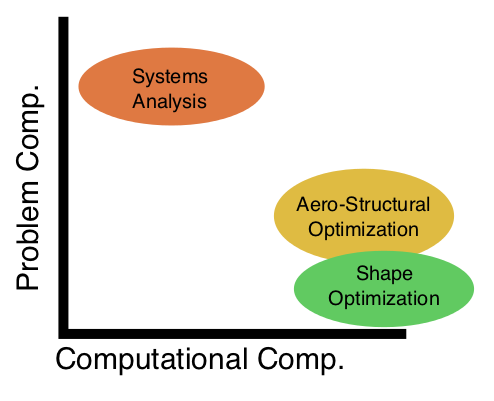
\includegraphics[width=.5\textwidth]{images/complexity_cartoon}
      \caption{ Notional spectrum of complexity in design problems currently being addressed. \label{fig:complexity_cartoon}}
    \end{center}\end{figure}

    In this work we demonstrate how OpenMDAO, an open-source framework, provides such a general
    solution to constructing and solving problems from across the complexity spectrum with large design spaces 
    using the same MDAO methods commonly applied to the the shape optimization and aero-structural optimization
    problems. OpenMDAO achieves this by providing three key features:

    \begin{enumerate}
      \item Automatic handling of arbitrary interdisciplinary coupling
      \item Automatic formulation of gradients, including coupled derivatives, given arbitrary coupling
      \item Efficient operation in a high performance computing environment with distributed data
    \end{enumerate}

    To demonstrate these capabilities, we present two different problem solved with 
    the OpenMDAO framework. The fist problem is the design of a small satellite 
    platform for taking weather measurements in the thermosphere, called CADRE. The CADRE problem has a
    medium problem complexity with about 20 disciplines and also medium computational complexity. 
    This problem demonstrates that OpenMDAO can efficiently solve problems with massive design spaced and 
    medium complexity. The second problem is an aero-structural design of 
    the Common Research Model wing, using CFD and FEA. This problem has very high computational 
    complexity and shows that OpenMDAO can be used effectively on problems that use higher fidelity 
    simulations, parallel execution, and distributed data. 

  \section{Dependency Graph}

    OpenMDAO maintains a monolithic data connectivity graph between all
    variables and components in the model, called the dependency graph.
    Using efficient graph traversal algorithms, OpenMDAO provides a number of
    features which make it easier to implement large scale design problems.

    \begin{itemize}
      \item Determination of component execution order via path finding.
      \item Identification of interdisciplinary coupling through cycle detection.
      \item Construction of a minimum-sized linear system to solve for gradients.
    \end{itemize}

    This section will describe the graph structure used to represent problem formulation in OpenMDAO,
    then discuss in detail how graph traversal algorithms are used to provide features. OpenMDAO relies
    on the NetworkX \cite{hagberg-2008-exploring} python package for implementation of each of
    the algorithms.

    \subsection{Graph Structure}
    The graph utilizes the structure proposed by
    Pate et. al \cite{graph_problem2013} and represents the complete problem formulation as
    defined by the user. In a dependency graph, each component and all variable inputs and outputs of that component are
    represented by nodes with directed edges between them describing their dependencies on each other.
    Figure \ref{fig:sellar_graph} shows a sample graph for the Sellar Problem \cite{AIAA:sellar}
    given in eqn. \ref{eqn:sellar_formulation}.


    \begin{align}
        \txt{given} & \ \ y_1 = D_1(x_1,y_2,z_1,z_2) \notag
        \\      & \ \ y_2 = D_2(y_1,z_1,z_2) \notag
        \\\txt{min.} &\ \ F(x_1,y_1,y_2,z_2) \notag
        \\\txt{w.r.t.} & \ \ x_1,y_1,y_2,z_1,z_2 \notag
        \\\txt{s.t.} & \ \ G_1(y_1) \geq 0 \notag
        \\     & \ \ G_2(y_2) \geq 0
        \label{eqn:sellar_formulation}
    \end{align}


    \begin{figure}[!htb]\begin{center}
      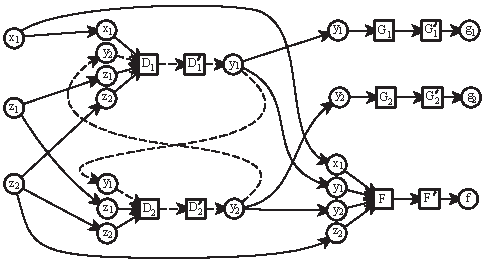
\includegraphics[width=.8\textwidth]{images/sellar_cycles}
      \caption{ Dependency graph for the Sellar problem. \label{fig:sellar_graph}}
    \end{center}\end{figure}

    In the original graph syntax, a single node is given for every variable. This holds true for the graph
    within OpenMDAO, with only one minor caveat. In the case of any hierarchical variables, such as arrays
    or VariableTrees, one variable node is created to represent the overall variable with additional nodes
    created if any specific sub-variable is referenced (e.g., some slice of an array or some child variable from a
    VariableTree). Figure \ref{fig:subvars} shows how the sub-variable nodes relate to their parent variables.

     \begin{figure}[!htb]\begin{center}
      xxxxxxx\\xxxxxxx\\xxxxxxx\\xxxxxxx\\xxxxxxx\\xxxxxxx\\
      \caption{ Example graph with child nodes for sub-variables \label{fig:subvars}}
    \end{center}\end{figure}

    By representing hierarchical data as a single node, we help keep the overall size of the graph manageable
    when large chunks of data are being communicated. However, if some small sub-set of that data needs to be
    used somewhere it is not correct to indicate a dependence on the entire chunk of data. So in this case, a
    single new node representing the sub-variable is created with its own dependence on the parent variable.
    This book keeping becomes particularly important for when the graph is used to calculate derivatives or
    manage the partitioning of distributed data. Both problems contain large design spaces. The CADRE problem 
    involves about 25000 design variables, and the aero-structural problem involves about 200. 
    Together these problems demonstrate how OpenMDAO can simplify the process of implementing difficult 
    design problems with large design spaces and varying kinds of complexity. 


    \subsection{Determining Execution Order}

    The OpenMDAO framework uses its dependency graph to determine component execution order by finding the 
    shortest path from the design variables to the quantities of interest for any given model\cite{openmdao_derivatives}. 
    This path contains the set of relevant components and variables that make up a sub-graph of the full
    dependency graph. During execution, only the components in this graph will be executed and they will be executed 
    in the order prescribed by following the graph path. 

    \subsection{Cycle Detection and Usage}
    Pate et. al indicate that within a dependency graph, the presence of cycles indicates coupling between
    the components in the cycle \cite{graph_problem2013}. A cycle can consist of two or more components, and
    one component may be part of more than one cycle.

    In formal terms, cycles exist in a graph when a group of nodes are strongly connected. The NetworkX package
    provides an implementation of Tarjans algorithm for finding sets of strongly connected
    components\cite{tarjan1972depth,nuutila1994finding}. Once found, the presence of these cycles
    have an impact on how any given model is solved. Firstly during normal execution, these cycles
    need to be converged with a numerical solver such as Gauss-Seidel or Newton based. 
    In addition these cycles need to be accounted for when solving for the gradients 

    \subsection{Gradient Calculation}
    
    OpenMDAO can calculate a gradient between any set of input and output nodes in the
    dependency graph by setting up the linear system devised by Martins and Hwang \cite{Martins2012} in their 
    work developing a unified theory for derivatives computation. 
    The requested derivatives are calculated from the solution of the set of equations that is assembled
    from the output-input derivatives of all the components. The number of equations 
    is determined by the number of variables represented the graph, which means that the linear 
    system can get very large. To allow for such large systems the full model Jacobian is implemented as 
    a linear operator, so that it never has to be stored entirely in memory. The
    linear operator takes a vector as input, and returns the product of the Jacobian with that vector.
    
    In Martins and Hwang's original work, they considered all possible variables in their linear system. 
    By using the dependency graph, OpenMDAO is able to achieve significant reductions computational cost of 
    solving the linear system. Using the same path finding algorithm for determining execution order, 
    OpenMDAO finds the reduced set of component nodes and variable nodes that are both downstream of the design parameters
    and upstream of a specific quantity of interest. One such sub-graph is found for each linear solve necessary to
    find all the derivatives of the system. It is possible that each sub-graph will contain different sets 
    of variables and components depending on the structure of the graph. Hence, each linear solve step 
    is kept to its minimum possible size to keep. 

    \section{Direct vs Adjoint Methods}

    OpenMDAO supports calculating derivatives in two ways: direct and adjoint. The direct method performs
    one linear solve for each design variable. The adjoint method performs one linear solve per each objective 
    and constraints. Hence, if you have more design variables than quantities of interest (as if often the case), 
    the adjoint method will require far fewer solves of the linear system. If you have fewer design variables then 
    objectives and constraints the forward mode is preferable. 

    OpenMDAO allows users to specify analytic derivatives of components by declaring one or more of the following three
    methods: 

    \begin{itemize}
        \item provideJ(ins, outs, Jacobian)
        \item apply\_deriv(input\_vector, result\_vector)
        \item apply\_derivT(input\_vector, result\_vector)
    \end{itemize}
    
    The provideJ method is the simplest method to implement, and also the most flexible. The user simply gives the framework the 
    Jacobian and the order of the columns and rows in that Jacobian. With that information, OpenMDAO can automatically 
    implement either the forward or adjoint derivatives methods. This flexibility comes with some computational cost however. 
    Although at the overall system level the Jacobian is provided as a linear operator, that linear operator is built out 
    of the set of component Jacobians which are all stored in memory. If your component has relatively few inputs and outputs 
    (on the order of 10's), then this cost is not likely to be significant. However, as the scale of the components grows, 
    the other two functions will offer better efficiency. 

    The two methods apply\_deriv and apply\_derivT implement Jacobian linear operators at 
    the component level for the direct and adjoint methods respectively. So the user must provide both if they 
    want the component to be able to operate in both forward and adjoint modes. If the user prefers one method over 
    the other, they can choose to only implement one or the other. When both methods are present OpenMDAO will 
    attempt to make an intelligent choice about whether to use the forward or adjoint method based on the number 
    of variables vs objectives and constraints. 
    
    \subsection{Mixed Analytic and Finite Difference Gradients}
    
    Many multidisciplinary systems contain a mixture of components that can provide their analytic derivatives, and
    those that cannot. OpenMDAO supports both of these types of component under the same umbrella of the
    solution method. When a component provides no derivatives, then the component is finite-differenced in-place to
    produce the derivatives that are used in the linear system of the full model. The dependency graph is also used
    to find groups of connected components with no derivative defined so that they can be finite differenced as a single entity. 
    
    To illustrate this: (figure)
    
  \section{CADRE Problem Formulation}

  The CADRE problem represents a class of problems with medium complexity and medium fidelity. 

    \begin{align}
        \\\txt{max.} &\ \ \sum_{i=1}^6 D_i \notag
        \\\txt{w.r.t.} & \ \ 0 \le I_{setpt} \le 4 \notag
        \\     & \ \ 0 \le P_{comm} \le 25 \notag
        \\     & \ \ 0 \le cellInstd \le 1 \notag
        \\     & \ \ 0 \le finAngle \le \pi/2 \notag
        \\     & \ \ 0 \le antAngle \le \pi \notag
        \\     & \ \ 0.2 \le iSOC \le 1 \notag
        \\\txt{s.t.} & \ \ I_{bat} - 5 \le 0 \notag
        \\     & \ \ -10 - I_{bat} \le 0 \notag
        \\     & \ \ 0.2 - SOC \le 0 \notag
        \\     & \ \ SOC - 1 \le 0 \notag
        \\     & \ \ fSOC - iSOC = 0 \notag
        \label{eqn:sellar_formulation}
    \end{align}


    \begin{figure}[!htb]\begin{center}
      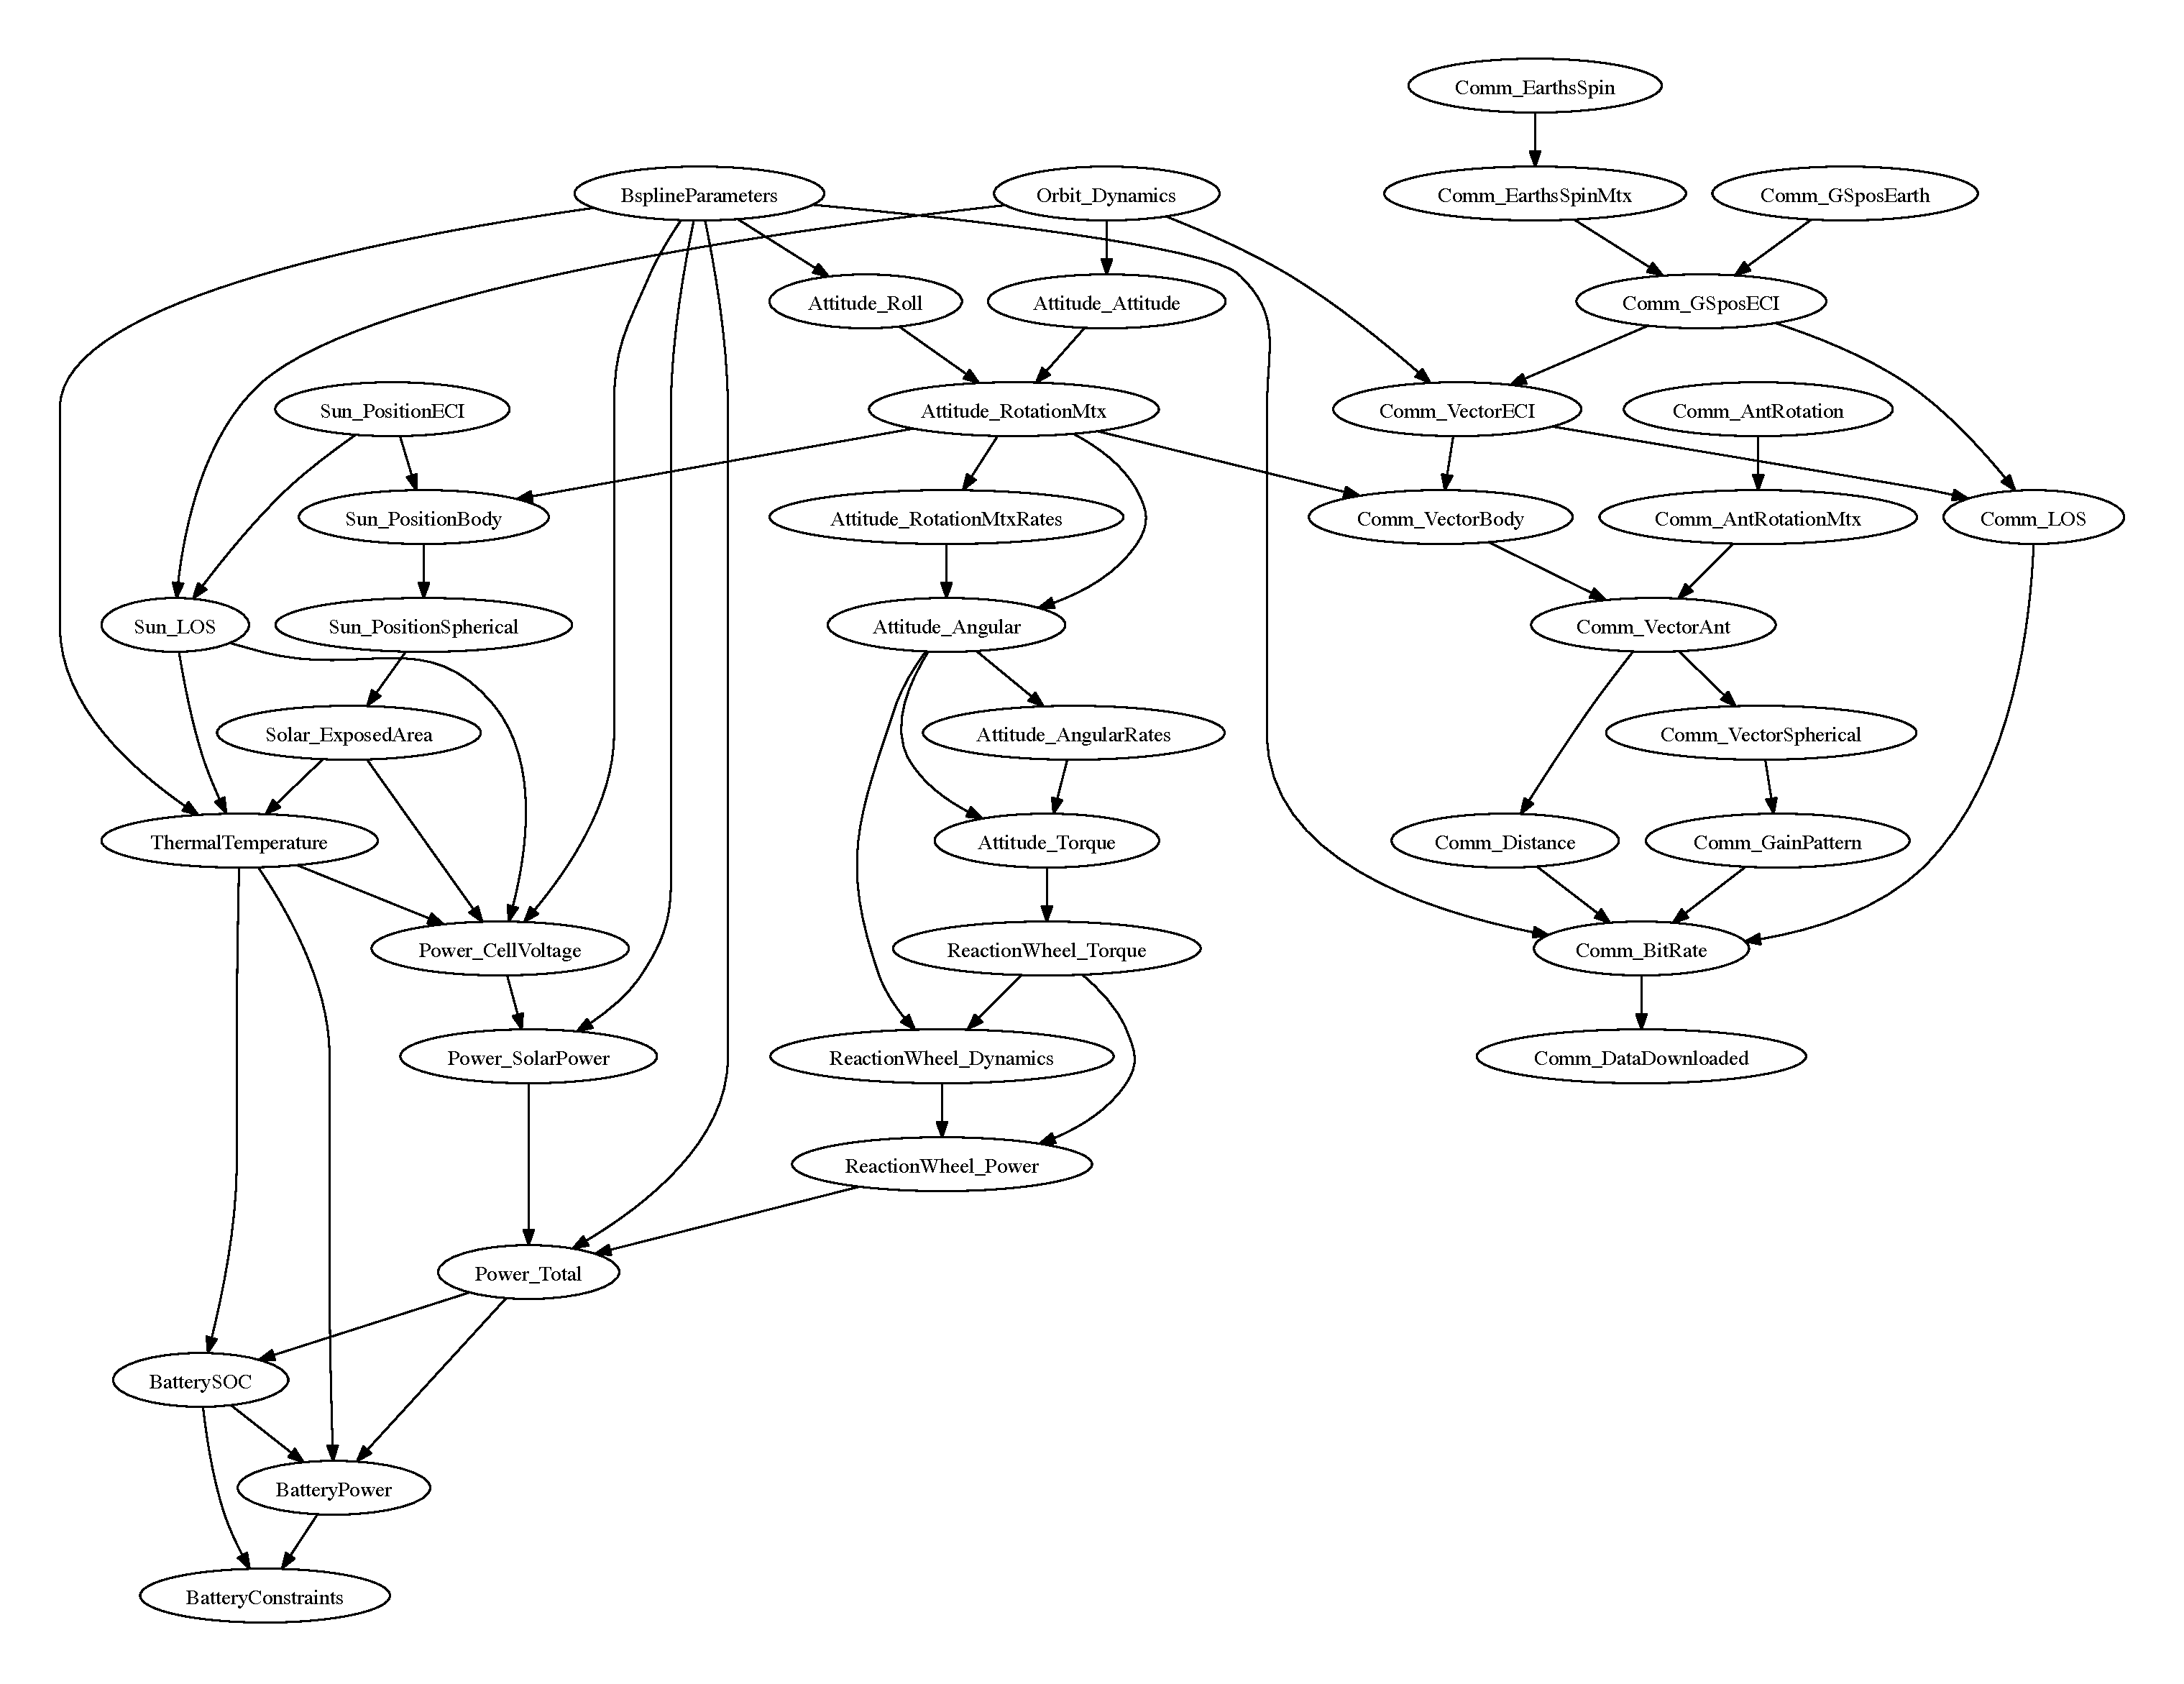
\includegraphics[width=1.1\textwidth]{images/CADRE.pdf}
      \caption{ Dependency graph for the CADRE problem. \label{fig:cadre_graph}}
    \end{center}\end{figure}

  \section{CADRE Results}

    The OpenMDAO implementation of the CADRE problem was executed on a 
    Macbook Pro (2.3 Ghz Core i7 processor, 4GB 1600 Mhz DDR3 memory, running OSX 10.8.5)
    over the course of two days, to a termination tolerance of $10^{-5}$. This tolerance
    was achieved within approximately 106 iterations, using the SNOPT\cite{gill2005snopt}
    optimizer.

    \begin{figure}
    \centering
    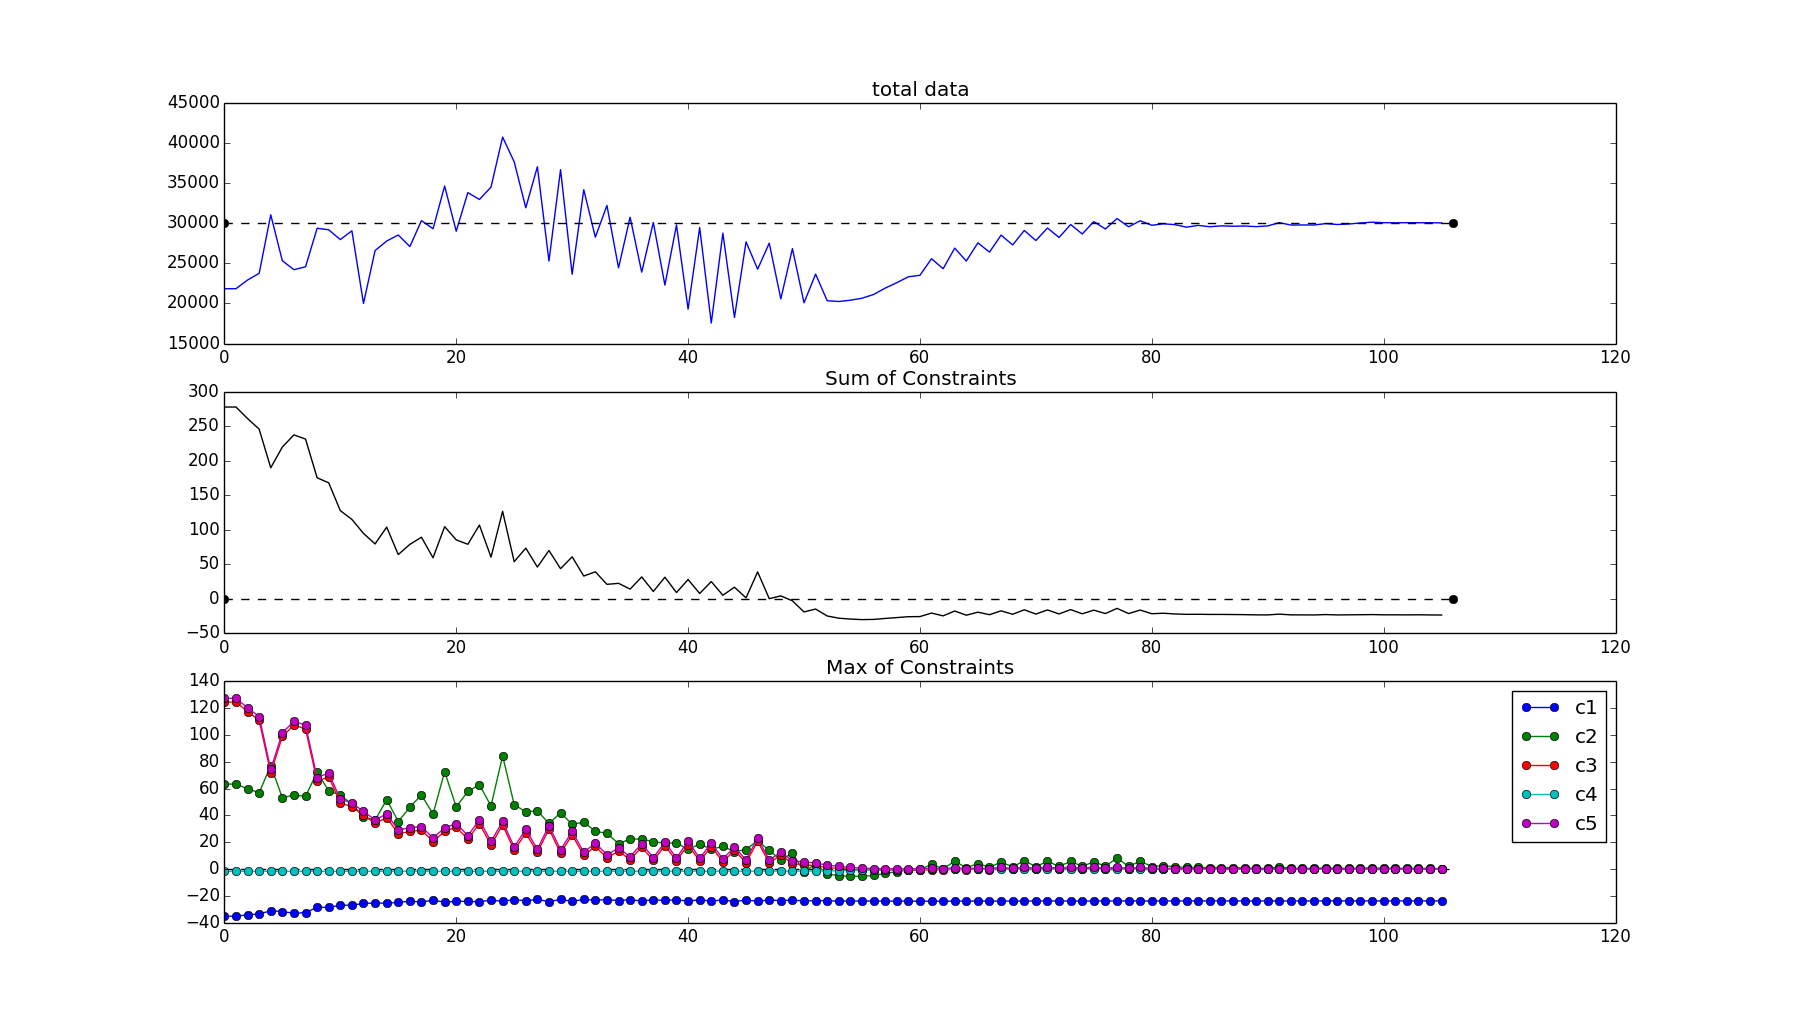
\includegraphics[width=0.99\textwidth]{images/opt.png}
    \caption[width=0.22\textwidth]{Convergence of the CADRE problem.}
    \label{convergence}
    \end{figure}


    Figure \ref{convergence} illustrates the convergence of the CADRE problem over the course of
    these iterations. The first row plots the
    value of the objective function, the total data downloaded over each design point. The objective
    function oscillated greatly over the course of the first half of the computed iterations, but
    stabilized by the 80th iteration near the value previously determined \cite{CADRE2012}
    to be the optimal design.

    The second row plots the maximum value of each constraint across all design points at
    each iteration. As all of the problem constraint are non-positive for a feasible design,
    this can be taken as a cursory measure of overall problem feasibility.
    The third row plots the maximum value of each constraint across each of the design points,
    but separated according to specific constraint type. These two plots both indicate that the
    oscillatory behavior of the objective function coincided with a steady decrease in design
    infeasibility. Once a feasible state was reached (near the 50th iteration), the optimizer
    began refining the design towards a more favorable value of the objective function.

    \begin{figure}
    \centering
    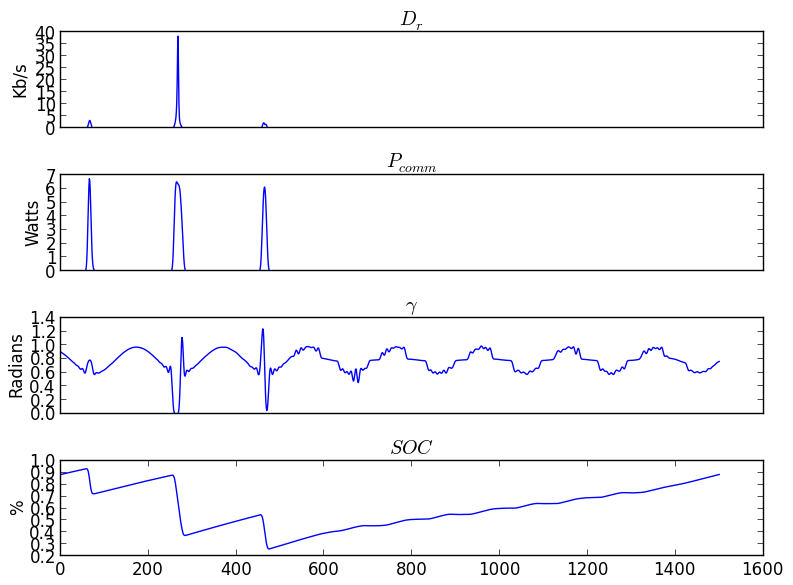
\includegraphics[width=0.8\textwidth]{images/pt_3_data.png}
    \caption[width=0.4\textwidth]{Plots of the bit rate, communications systems power, craft roll angle,
    and battery charge level over the half-day time period covered by the $4^{\textrm{th}}$ design point.}
    \label{pt3_data_results}
    \end{figure}

    Figure \ref{pt3_data_results} shows plots of selected variables for the $4^{\textrm{th}}$ design point,
    to illustrate the fidelity of the recovered solution. These variables are the communications 
    bit rate ($D_r$), communications systems power level ($P_{comm}$), craft roll angle ($\gamma$),
    and battery charge level ($SOC$). Prior to the optimization, these variables
    were each instantiated to uniform values
    (across all time points) of 0, 0, $\frac{\pi}{4}$, and 0 respectively. The optimizer, operating on
    OpenMDAO's graph formulation of the problem succeeded at converging each of these variables to the values
    shown, for each time point. Line of sight is seen to have been achieved in three short ranges of time near the
    beginning of the modeled half-day design point. Interestingly, though the data rate achieved in the second
    time period with affirmative line of sight is significantly higher than the other two periods, the optimizer
    converged to a solution that provided power to the communications system near uniformly for each of these
    three time periods.

    Figure \ref{pt3_data_results} shows that the craft roll angle, $\gamma$, roughly approximates a sine function
    with a wavelength of 90 minutes (the approximate orbital period of the satellite),
    with short term perturbations during the time
    periods where line of sight is gained with the ground station. That is, the optimizer successfully
    converged to a solution with the satellite continuously turned to maximize exposure to the sun,
    except when turning to point its antenna towards the ground station during times when
    communication is possible. This dynamic is also reflected in the battery state of charge ($SOC$)
    data plotting in the bottom row, with the battery losing charge quickly during
    communication with the ground station, but recharging while tracking with the sun.

    Further post processing of the data included automatic geographical rendering of the trajectories of
    the CADRE satellite for each of the 6 design points, using the Google
    Maps\footnote{http://developers.google.com/maps/} and Google
    Earth\footnote{http://developers.google.com/earth/} APIs. The trajectories are
    represented as polygonal chain ("polyline") elements, colored according to the
    satellites communication bit rate with the ground station during the corresponding
    window of time. Each colored line segment are centered on the locations
    determined by the time points when the data bit rate values were calculated
    by the OpenMDAO model.

    Figure \ref{pt3_g_earth} communications bit rate along the trajectories of the
    CADRE satellite during the $4^{\textrm{th}}$ design point. This can be compared
    directly with Figure \ref{pt3_data_results}, where one large spike in communications
    bit rate was preceded and then succeeded by two short time periods of lesser
    data rates. Plotted geographically, this is seen to be due to the procession of
    the satellites orbit, where the period of maximal data rate corresponds to a
    pass of the satellite directly over the ground station location. The proceeding and
    succeeding data rate spikes correspond to passes over the near Atlantic and
    Rocky Mountain regions, respectively.


    Figure \ref{allpt_flatmap} similarly shows trajectory and bit rate data plotted
    from all six design points, centered on the United States. The orbital passes
    that are close enough to the ground station for communications can all be seen.
    Figure \ref{allpt_g_earth} zooms this view out to show coverage of the trajectories
    of all design points across the Earth.


    \begin{figure}
    \centering
    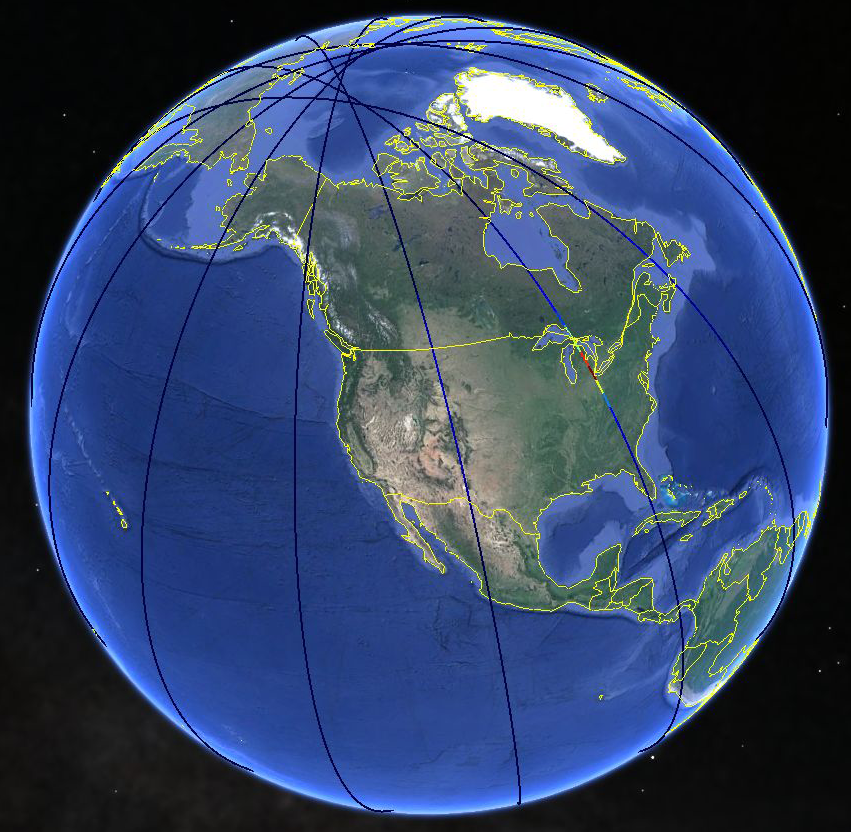
\includegraphics[width=0.8\textwidth]{images/pt3_gearth3.png}
    \caption[width=0.4\textwidth]{Plot of the trajectories of the CADRE satellite
    for the $4^{\textrm{th}}$ design point onto the surface of the Earth, illustrating the
    communication data rates near the ground station.}
    \label{pt3_g_earth}
    \end{figure}


    \begin{figure}
    \centering
    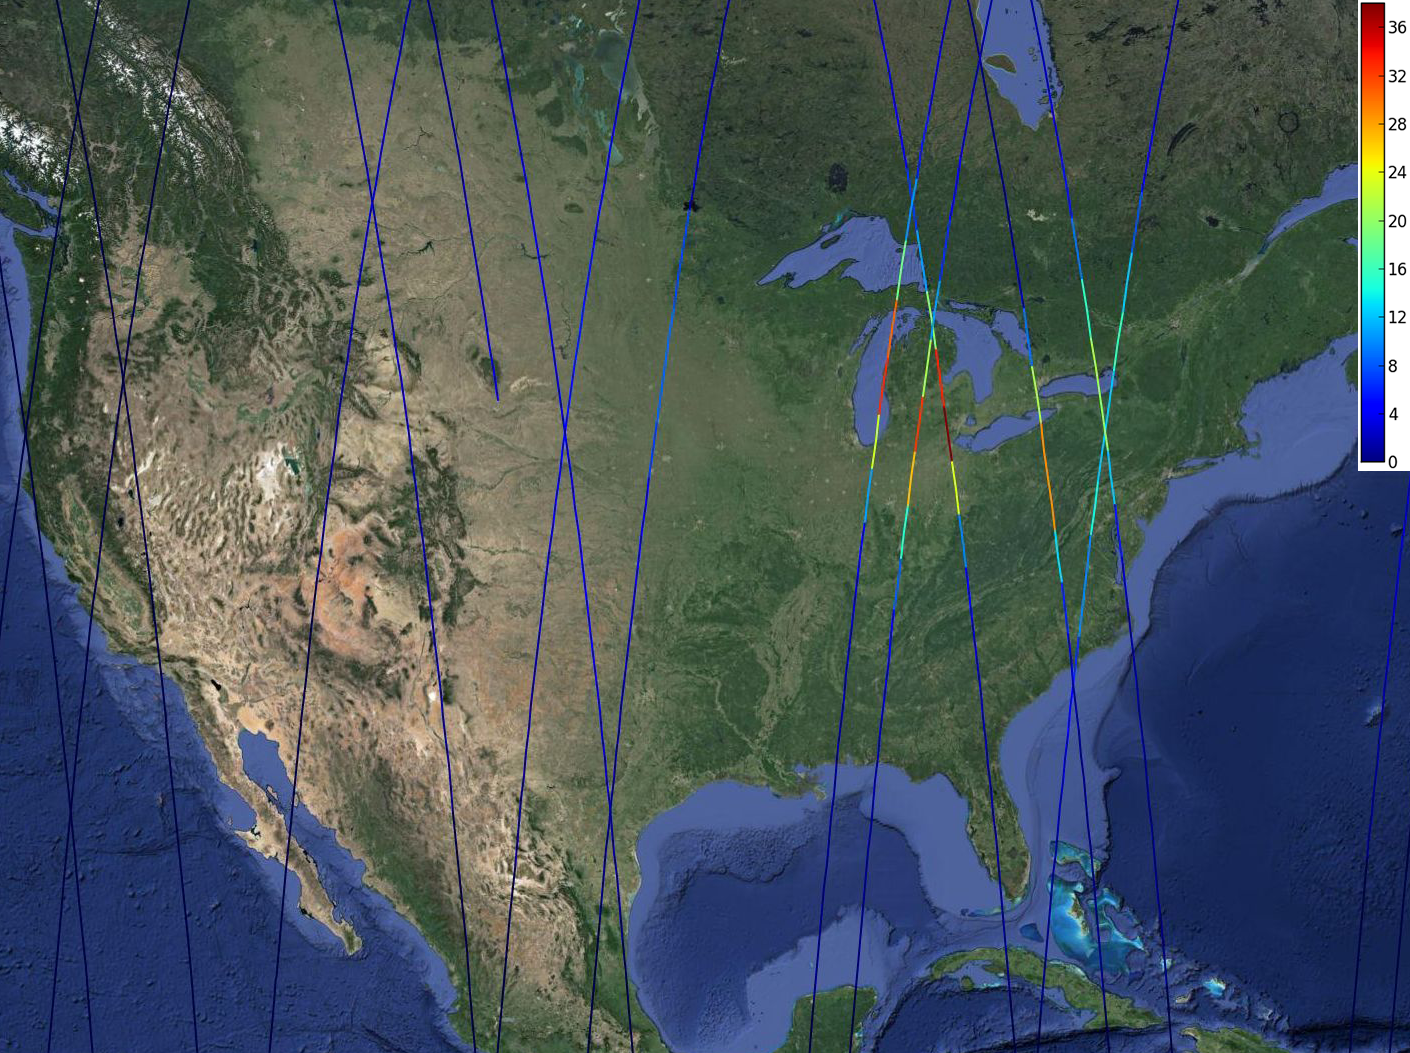
\includegraphics[width=0.8\textwidth]{images/allpts_map_data.png}
    \caption[width=0.4\textwidth]{Plot of the trajectories of the CADRE satellite
    for all 6 design points onto the surface of the Earth, illustrating the
    communication data rates near the ground station.}
    \label{allpt_flatmap}
    \end{figure}


    \begin{figure}
    \centering
    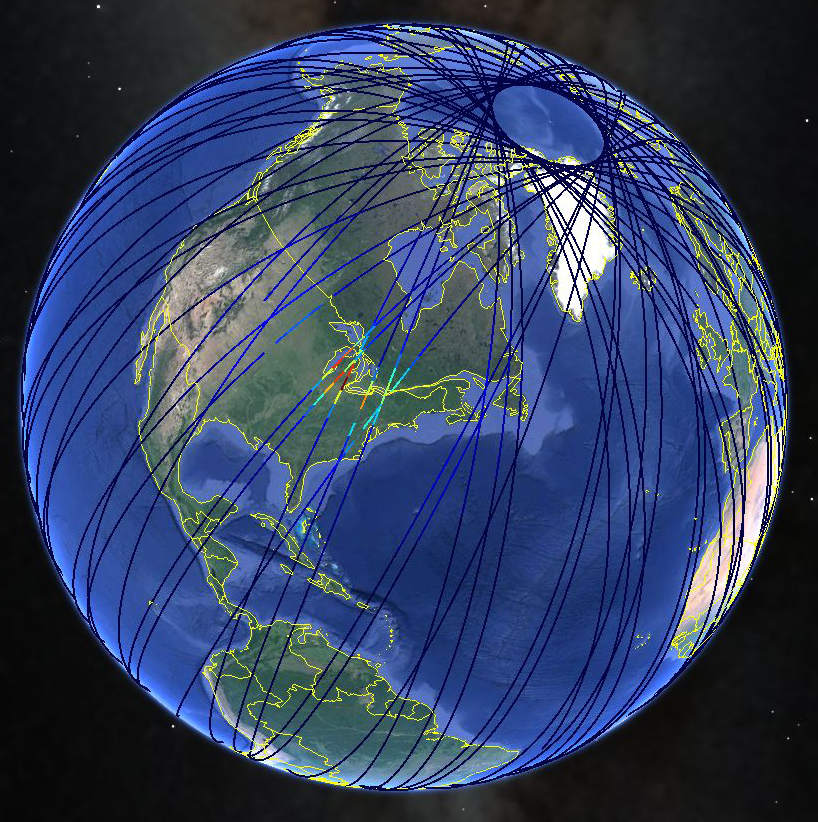
\includegraphics[width=0.8\textwidth]{images/allpts_gearth2.png}
    \caption[width=0.4\textwidth]{Plot of the trajectories of the CADRE satellite
    for all 6 design points onto the surface of the Earth.}
    \label{allpt_g_earth}
    \end{figure}


  \section{Aero-Structural Problem Formulation}

  \section{Aero-Structural Results}

  \section{Conclusion}

  \bibliography{references}


\end{document}
